\documentclass[a4paper]{article}

\usepackage[utf8]{inputenc}
\usepackage{blindtext}
\usepackage{setspace}
\usepackage{microtype}
\usepackage{graphicx}
\usepackage{wrapfig}
\usepackage{amsmath}
\usepackage{index}
\usepackage{enumitem}
\usepackage{geometry}
\usepackage{fancyhdr}
\usepackage{tabularx}
\usepackage{multirow}
\usepackage{multicol}
\usepackage{array}
\usepackage{biblatex}
\usepackage[T1]{fontenc}
\usepackage{hyperref}
\usepackage{parskip}
\geometry{left=2.7cm,right=2.7cm,top=2.7cm,bottom=2.7cm}
\graphicspath{{images/}}

\usepackage[dvipsnames]{xcolor}
\hypersetup{colorlinks=true, linkcolor=RoyalBlue, urlcolor=RoyalBlue}

\title{
    \vspace{5em}
    \textbf{\huge E-Fuels Notes}
    \large}
\author{Riddhiman Roy}
\date{Summer 2021}
\onehalfspacing
\begin{document}

\maketitle
\thispagestyle{empty}

\setcounter{page}{0}

\begin{centering}
\section*{Introduction}
These are notes compiled by Riddhiman Roy for the E-Fuels Project as part of ESROP-UofT during the summer of 2021. They will contain notes from papers to be read and discussed as part of the aforementioned project. If there's anything wrong, reach out to me \href{https://riddhimanroy.com/contact.html}{here.}
\end{centering}

\tableofcontents
\pagebreak

%%%%%%%%%%%%%%%%%%%%%%%%%%%%%%%%%%%%%%%%%%
\section{Technological and Methodological Overview of Various\\ Power-to-X Systems}
\subsection{Overview}
This paper, written by Koj et.al (available \href{https://www.sciencedirect.com/science/article/pii/S1364032119304228}{here}) conducts a review of 32 LCA studies on various Power-to-X chains. It compares "influencing factors on environmental impacts"[1]. According to its abstract, it considered various studies which featured chains such as Power-to-Gas, Power-to-Transport, Power-to-Power, Power-to-Liquids and Power-to-Chemicals.

\subsection{Definitions}
\begin{itemize}
    \item \textit{Power-to-X}: While there is no definite definition, the paper defines it as "process chains for the conversion of electricity into various products or applications and their associated technological components." The paper also distinguishes between the individual phases of the process, seperating "Power", "to" and "X."
    \item \textit{Power}: In the context of energy use scenarios, it is usually assumed that this power (for the input stage of various Power-to-X chains) comes mostly or entirely from renewable sources. Furthermore, this stage would also include the means of connection into the Power-to-X chains ("isolated solutions vs grid connections").
    \item \textit{To}: This phase describes the intermediate processes and inputs (in most cases, carbon dioxide and water). It also includes transportation and distribution components which are prerequisite in infrastructures.
    \item \textit{Well-to-Wheel}: This describes the comprehensive use of energy resources and emissions that accumulate from the point of fuel source extraction to utilization in a vehicle.
\end{itemize}
\subsection{Power-to-X chains}
    \begin{itemize}
        \item The paper stresses the impact considering the integration of all systems within the power-to-x chain as influential to the environmental impact and performance of the chain.
        
        \item Water is a very common input into various chains. It is decomposed into hydrogen and oxygen using electrolysis, of which there are two competing technologies: AEL (alkaline water electrolysis) and SOEC (solid oxide electrolysis). To get 1kg of hydrogen, both processed require 10L deionized water input and 18L of proton exchange membranes (PEMs).
        
        \item If PEM or AELs is used (low temperature electrolysis), then carbon dioxide efficiency in various power-to-x process chains go from $38\% to 41\%$ when it is sourced from ambient air, and from $47-51\%$ to $53\%$ when sources from biological sources. 
        
        \item Still, the paper notes that often, the limiting factor in carbon dioxide sources are availability restrictions and separations costs. However, these were not further assessed in the paper.
        
        \item Some power-to-x chains can be operated independent of grid boundaries, leading to reduced loads on the grid. However, most do not operate this way. Most require transportation of sources such as water and carbon dioxide. The paper stresses that in most cases, such transportion is necessary. 
        
        \item Storage is also important for such chains, especially for gaseous components. It proposes the use of large underground tanks for storage of high energy density gasses.
    \end{itemize}
\subsection{Product Groups}
    \begin{itemize}
        \item \textit{Power-to-Gas}: Hydrogen is often considered one of the most common inputs for most chains and often, Power-to-gas can lead to hydrogen. 
        \begin{itemize}
            \item AEL, PEM and SOEC are considered to be the most talked processes for hydrogen production
            \item AEL is considered to be the most able to cope with VRE sources as well as the most mature and cheapest technology.
            \item SOEC is the most expensive and least ready technology, however it is expected to have the highest efficiency.
            \item PEM is the most flexible technology with short startup times and fast response times.
        \end{itemize}
        \item \textit{Power-to-methane}: This chain outlines the process of converting hydrogen to methane in a methanation reaction with carbon dioxide, leaving methane and water vapour. Synthetic natural gas can be produced upon refinement.
        \begin{itemize}
            \item Methanation processes: Thermochemical methanation typically has lower efficiency rates compared to biological methanation with efficiency rates ranging from 70 to 85\% compared to the peaks of 98\% for biological methanation. However, it is more mature than biological methanation with a TRL between 5 and 7.
        \end{itemize}
        \item \textit{Power-to-syngas}: Besides regular gas, power-to-syngas also exists. There are 4 main processes: steam reformation, reverse water gas shift reaction (rWGS), dry reforming of methane (DRM) and co-electrolysis. However, syngas is usually an intermediate.
        \item \textit{Power-to-liquids and power-to-chemicals}: Liquid energy carriers are generally produced for transportation and chemical fuel needs. Power-to-liquids are closely connected to power-to-fuels and power-to-chemicals. Conversion processes include the Fischer-tropsch and methanol synthesis.
    \end{itemize}
\subsection{Applications}
\begin{itemize}
    \item \textit{Power-to-heat}: This heat, often a by-product of other chains (such as themochemical methanation for power-to-methane), is used for residential and industrial purposes. To convert electricity into heat, electric broilers and heat pumps are used, the latter having larger variance and an ability to integrate ambient heat into production compared to the former.
    \item \textit{Power-to-transport}: The paper considers Fuel Cell Vehicles (FCVs), Battery Electric Vehicles (BEVs) and Internal Combustion Engine Vehicles (ICEVs) (if using methanol or syngas) to be promising applications for Power-to-transport applications. The paper assumes that in BEVs, electricity is consumed immediately, without intermediate processes.
    \item \textit{Power-to-power}: This application centers around converting power into a gaseous product, transporting then using it again as electricity. In Europe, such products are typically hydrogen.
\end{itemize}
\subsection{Methodological Analysis}
The paper discusses that there exist a variety of scopes, key technological parameters and methodological choices. Below are some key highlights.
    \begin{itemize}
        \item 19 studies use an energy related functional units, while 11 use distance related functional units (1 km). However, a majority of the studies using distance related functional units do not state an expected VKT over the lifetime of their vehicles.
        \item 17 of the studies limit their chains at the product (methane at a power-to-methane chain). However, only 6 consider the use of those products in some application such as transportation. 3 more are wheel-to-well studies. However, wheel-to-well studies do not consider the energy conversion and vehicle technologies.
        \item Between papers, there were major differences in between the operation and construction phase of the lifecycle of various chains.
        \begin{itemize}
            \item Most studies included more data concerning the operational phase of power-to-x chains compared to the construction phase. 24 out of the 32 considered did not include any LCI data concerning the construction phase. 
        \end{itemize}
        \item There are no consequential LCA of power-to-x published, however, all of these studies perform attributional LCA.
        \item The most commonly used database is ecoinvent, followed by GaBi, GREET and GEMIS. However, the paper regards the use of ecoinvent in some papers as outdated since ecoinvent3 was launched in 2013.
        \item While most studies (23) focused on contemporary timeframes under current conditions, nine focused on the near future (2020), while 7 discussed long term (2050) development.
        \item There is a significant focus on European grids and markets - especially Austria, Germany and Switzerland. The EU as a whole is also discussed.
        \item 21 studies considered various grid mixes, followed by wind for electricity input. \item For electrolysis, AEL and PEM are almost equally prevalent. SOEC is only considered in 3 studies.
        \item 12 studies focus on gas products, followed by liquid (especially methanol) considered by 14 studies. 1 study focussed on chemical products.
    \end{itemize}
\subsection{Life Cycle Assessment Results}
\begin{itemize}
    \item Hydrogen produced in power-to-gas or power-to-syngas can be a part of other power-to-x chains and other hydrocarbon products.
    \item Hydrogen production from renewable sources leads to lower emissions and impacts compared to traditional sources of energy. Wind energy is especially potent, observed in studies where geography and grid mixes on various levels are considered, at reducing impacts.
    \item One LCA process used was "vehicle \& road," with construction, maintenance, abrasion and road wear components.  
    \item For power-to-hydrogen chains, the source of electricity significantly affects the impacts of the chain.
    \item FCVs with hydrogen or syngas with electricity sources from the grid can cause higher climate change impacts compared to ICEVs.
    \item Zero emission vehicle (ZEVs) is problematic since the classification only considers direct emission impacts from the operation of the vehicle, without consideration of the source of the fuel used nor power-to-x chain used. 90\% of the impact is a result of fuel production processes.
    \item For solar cells, PV technology also plays a part. Cadmium Telluride cells cause 30g of equivalent carbon dioxide per km less compared to polysilicone cells.
    \item While current ICEV-Gs emit in the range of 100-160g of equivalent carbon dioxide per km. However, this is expected to improve due to political pressure.
    \item For power-to-heat, it was found the emission reduction potential was highly dependent on the COP of heat pumps.
    \item The use of steel and aluminium for wind turbines and PV cells are identified as important considerations for human toxicity analysis. In addition, copper and fossil fuels are also important if a mixed grid is used for energy sources.
    \item Power-to-methanol plants are generally found to be environmentally better and perform well in all impact categories compared to natural gas, syngas and biomass based plants.
    \item The study by Koj et.al concluded that when surplus energy is used, ozone depletion is negatively impacted due to the use of PTFE for gaskets of electrolyzers. Nickel use has also been found to have negative impacts through increased acidification.
    \item For FCVs, as detailed by Tshiggerl et al., aluminium, platinum, steel, carbon fibre and PTFE (materials in fuel cells) are found to have significant contributions to their impacts.
    \item If wind is the electricity source, then power-to-chemical chains are found to be least electricity intensive of the traditional paths to the same chemicals. However, they are the most materially intensive.
    \item If seperation costs are included, then carbon dioxide emission from seperation in fossil fuels is greatly increased, with a 4x increase for power-to-methane and 14x increase for power-to-methane-to-transport.
\end{itemize}
\pagebreak
\subsection{Figures}
\begin{figure}[h!]
    \centering
    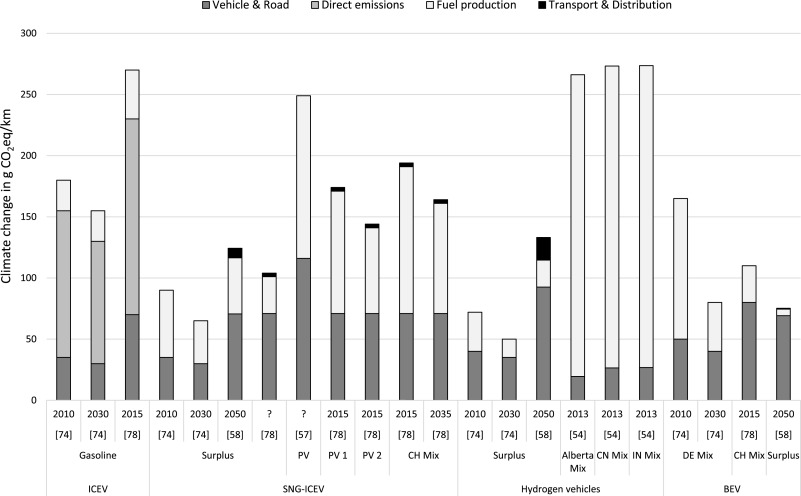
\includegraphics[scale=0.7]{hydrogen emissions vs grid mix and transport type.jpg}
    \caption{Climate Change impact from production of hydrogen in power-to-transport chains, by regional and national grid mixes and vehicle technology.}
    \label{fig:1}
\end{figure}
\begin{figure}[h!]
    \centering
    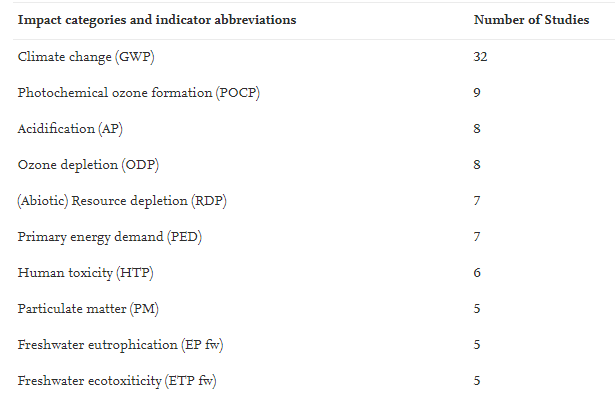
\includegraphics[scale=0.7]{impact area breakdown.PNG}
    \caption{Breakdown of the impact area discussed in the studies analyzed.}
    \label{fig:2}
\end{figure}
For more detailed breakdown of the studies and their properties in tabular form, consult the paper directly.
\end{document}
